\chapter{Environnement de travail}
\label{sec:EnvironnementDeTravail}

L'objectif de ce chapitre consiste à expliciter tous les éléments relatifs à l'environnement logiciel sur lequel j'ai travaillé pour réaliser cette application. Il s'agit donc des logiciels, langages, frameworks, et motifs d'architecture auxquels j'ai fait recours tout au long du processus de mise en œuvre de ma solution.

\section{Gestion du projet}
Dans cette section, je présente la méthodologie de travail et le logiciel de gestion de projet que j'ai utilisé pour déclencher, organiser et gérer le travail sur ma solution.

\subsection{Méthodologie de travail}
C'est la manière de mener un processus de développement. Il s’agit d’une démarche, un ensemble d’étapes ou procédures à mettre en œuvre dans une logique méthodologique, accompagnés d’outils et de techniques. L'utilisation d'une méthode est incontournable dans l'entreprise de tout projet, particulièrement dans la réalisation de projets informatiques. Dans ce cas-ci, les méthodes utilisées sont des méthodes d'analyse et de conception qui ont pour but la formalisation des étapes préliminaires au développement de systèmes logiciels, en d'autres termes : analyse, modélisation et conception. \newline
L'urgence de l'utilisation de ces méthodes trouve son explication dans un certain nombre de facteurs :
\begin{enumerate}
	\item De nombreux échecs de projets informatiques dans le passé dus à un manque d'organisation, ou une non satisfaction des besoins ;
	\item La révolution de l'industrie logicielle engendrée par les échecs informatiques et qui introduit de nouveaux facteurs de validation de la
		qualité logicielle : le génie logiciel ;
	\item Les nombreuses exigences liées au coût, aux délais et à la complexité des projets informatiques.
\end{enumerate}
L'utilisation de méthodes de développement de logiciels permet ainsi l'élaboration de systèmes informatiques de manière fiable et viable tout en répondant à l'ensemble des exigences du client et du génie logiciel.
\newline \newline
Il existe plusieurs méthodes de développement informatique. L’on distingue deux approches : l’approche traditionnelle et l’approche agile. Les deux approches se distinguent essentiellement dans la manière de décomposer le projet. Les méthodes cartésiennes ou fonctionnelles ou encore traditionnelles se sont imposées les premières.
\subsubsection{L'approche traditionnelle}
Cette approche s’inspire directement de l’architecture des ordinateurs. Les méthodes traditionnelles prônent une démarche strictement planifiée avec une séquence d’activités bien définie. La succession des activités et le planning doivent être clairement respectés et aucun changement n’est permis. Il est attendu du client une spécification des besoins globale, détaillée, claire, précise et validée en entrée. Ainsi, tout doit être prévisible, du début du projet à la livraison du produit, d’où l’appellation de méthodes prédictives. \newline
Selon le planning adopté, les méthodes cartésiennes proposent plusieurs modèles d’exécution des activités du projet :
\begin{enumerate}
	\item Le \textbf{modèle en cascade} : dans ce modèle, le processus de développement est découpé séquentiellement et de façon linéaire selon les activités intrinsèques du cycle de vie du développement logiciel : l’analyse, la conception, le codage et les tests. Le plan de déroulement des phases (planification prédictive) est élaboré en tout début de processus. Le passage à une phase donnée n’est fait que si le résultat de la phase précédente a été validé et jugé satisfaisant par le client et les utilisateurs.
	\item Le \textbf{modèle en V} : Le cycle en V est à la base de tout développement logiciel, il en représente les activités intrinsèques. Il tient d'avantage compte de la réalité que le modèle en cascade, le processus de développement n’est pas réduit à un enchainement de tâches séquentielles. Le modèle en V permet d’anticiper sur les phases ultérieures de développement du produit en particulier les plans de test de qualifications et de performance.
\end{enumerate}
Parmi les méthodes traditionnelles, nous pouvons citer : SADT, CORIG, …
\subsubsection{L'approche agile}
Cette approche est définie par les concepts suivants : la simplicité, la légèreté, la souplesse, un lien fort avec le client. C’est dans cette optique que certains apparentent le développement agile aux notions de flexibilité, de rétroaction et d’adaptation au changement rapide et continu.
\newline
Une méthode agile est une approche itérative et incrémentale, qui est menée dans un esprit collaboratif avec juste ce qu’il faut de formalisme. Elle génère un produit de haute qualité tout en prenant en compte l’évolution des besoins des clients et en anticipant sur les risques. Il y’a continuellement des aller et retour avec le client. L’application logicielle est livrée par version incrémentale. Les versions successives sont aussi fiables que le livrable final en termes de tests et de validation. En quelque sorte le processus est déroulé comme un enchaînement de « mini-cascades ». A chaque nouvelle itération, l’ensemble de l’architecture et de la conception logicielle est reconsidéré, le code est retravaillé.
\newline
Les méthodes agiles aspirent donc à améliorer la réactivité et l’adaptabilité des sociétés de logiciels et constituent un moyen de survie dans un environnement instable en s’accompagnant des valeurs suivantes :
\begin{enumerate}
	\item Les individus et les interactions plutôt que les processus et les outils;
	\item L’application fonctionnelle plutôt que la documentation compréhensive;
	\item La collaboration avec le client plutôt que la négociation des contrats;
	\item La réponse au changement plutôt que le suivi d’un plan.
	\newline
\end{enumerate}
L’agilité comprend plusieurs courants de pensée qui ont conduits à des méthodes différentes, reposant sur les mêmes concepts mais présentant des singularités. Les méthodes Scrum, Kanban, et XP (eXtreme Programming) sont des exemples de ces méthodes.
\newline\newline

\textbf{La méthode SCRUM}
\newline
\textbf{Scrum} est une méthode agile de gestion de projet qui permet de produire la plus grande valeur métier dans la durée la plus courte. Elle a pour objectif d’améliorer la cohésion de l’équipe et la rapidité du processus de développement. Le nom Scrum renvoie à une pratique généralement connue au rugby signifiant la « mêlée ». \newline
Cette méthode qualifie un ensemble de rôles, d’instruments de gestion et de pratiques managériales favorisant un environnement basé sur la transparence, l’inspection, le suivi et l’adaptation. Le cycle de vie d’un projet Scrum peut être découpé en trois parties :
\begin{enumerate}
	\item Phase d'\textbf{initiation ou démarrage} : il s’agit d’une phase linéaire où l’on définit le périmètre fonctionnel du système et la liste des fonctionnalités (\textbf{Backlog}) agencées par ordre de priorité, d’effort, de complexité et de risque. C’est aussi à ce niveau que l’architecture est définie.
	
	\item Phase de \textbf{développement} est un processus empirique : le projet est découpé en cycles itératifs d’une durée de deux semaines ou \textbf{sprints}. Chaque sprint regroupe une ou plusieurs fonctionnalités du Backlog. Tout au long de cette phase, le travail réalisé est mesuré et contrôlé et une amélioration constante du prototype est faite.
	
	\item Phase de \textbf{Clôtures} est une phase linéaire de gestion de la livraison du produit final.
\end{enumerate}
La figure \ref{Scrum} montre l’articulation générale de Scrum. \newline
\begin{figure}[h]
	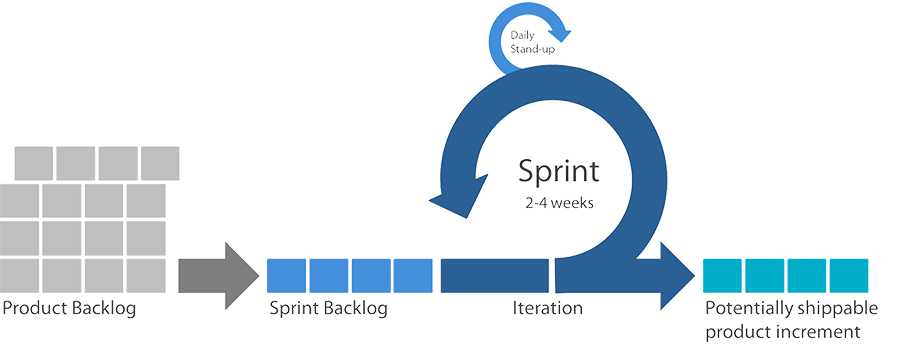
\includegraphics[width=18cm, height=9cm]{Images/scrum}
	\centering
	\caption{Articulation générale de la méthode Scrum}
	\label{Scrum}
\end{figure}
Les responsabilités managériales sont réparties sur trois rôles fondamentaux :
\begin{enumerate}
	\item \textbf{Scrum Master}
	\item \textbf{Product Owner}
	\item \textbf{Équipe Scrum}
	\newline
\end{enumerate}
Les artéfacts et pratiques de Scrum
\begin{enumerate}
	\item \textbf{Product Backlog} : état courant des tâches à accomplir;
	\item \textbf{Sprint} : itération de deux semaines;
	\item \textbf{Effort-Estimation} : permanente sur les entrées du Backlog;
	\item \textbf{Sprint Backlog} : Product Backlog limité au sprint en cours;
	\item \textbf{Daily Scrum Meeting} : ce qui a été fait, ce qui reste à faire;
	\item \textbf{Sprint Review Meeting} : Présentation des résultats du Sprint. \ref{Scrum}
	\newline \newline
\end{enumerate}

\textbf{SCRUM contre KANBAN}
\newline
Scrum est plus prescriptif que Kanban, qui évite de définir les rôles et les équipes et qui n’a pas de structure formelle de réunions. Kanban ne prescrit pas non plus d’itérations – bien qu’elles puissent être incorporées si vous le souhaitez. \newline
Les techniques de visualisation des processus de Kanban le rendent idéal pour les équipes colocalisées qui travaillent sur un backlog d’éléments sujets à des changements fréquents (par exemple, Kanban est souvent utilisé par les équipes de support). \newline
Le tableau Kanban est cependant souvent adopté par les équipes Scrum sous la forme d’un tableau de tâches et est utilisé pour suivre la progression tout au long d’un sprint. \newline
La limite de la règle Work In Progress dans Kanban la rend également adaptée aux équipes ayant des ressources limitées ou lorsque l’entrée de chaque membre est requise sur chaque élément. Cela pourrait s’appliquer, par exemple, à une équipe de communication au sein d’une grande organisation. \newline
Alors que Scrum limite la quantité de travail dans chaque sprint, la charge de travail est déterminée par l’estimation relative de la taille de chaque histoire (en points) et est approuvée par l’équipe Scrum à chaque session de planification. \newline
Alors qu’une équipe Kanban suit le « temps de cycle » et optimise les délais d’exécution aussi courts et prévisibles que possible, une équipe Scrum vise à améliorer son rendement sur les sprints successifs et à améliorer la « vélocité » de l’équipe (le nombre de points d’estimation relatifs complétés dans un sprint). Cela rend sans doute Scrum plus adapté à la mise à l’échelle – il semble certainement plus familier et prévisible, ce qui peut être rassurant pour les grandes organisations. \newline\newline

\textbf{SCRUM contre XP}
\newline
Dans Scrum, les équipes et les réunions sont assez gravées dans le marbre \footnote{Dans l’antiquité, les engagements pour la constructions de bâtiments importants étaient gravés sur des plaques de marbre (Athènes : arsenal du Pirée, Delphes). Les travaux s’étendant sur de nombreuses années, on ne pouvait faire confiance aux tablettes de cire ou aux papyrus. Sur ces plaques, on définissait par exemple la grandeur du bâtiment ou le montant des amendes pour les retards. Ce qui n’était pas « gravé dans le marbre » n’était donc pas contractuel. Voir le lien \href{https://fr.wiktionary.org/wiki/graver_dans_le_marbre}{https://fr.wiktionary.org/wiki/graver-dans-le-marbre}} alors que la question de savoir comment le travail est réellement fait est laissée aux équipes pour décider elles-mêmes. XP, d’autre part, est livré avec un ensemble de pratiques de base qui pourraient sembler accablantes pour le débutant Agile. \newline
On pourrait dire que Scrum est une méthodologie, qui est plus concernée par la productivité tandis que XP est plus préoccupé par l’ingénierie. \newline
La valeur que les pratiques XP peuvent ajouter est incontestable et de nombreuses organisations qui utilisent Scrum adoptent la programmation par paires, le développement piloté par les tests et le refactoring comme des pratiques qui améliorent la qualité, accélèrent le processus de publication et / ou réduisent le besoin de revoir le travail en raison de la dette technique. \newline
Outre les itérations plus courtes, d’autres éléments importants qui différencient XP de Scrum sont les suivants :
\begin{enumerate}
	\item Les équipes XP travaillent sur des éléments dans un ordre de priorité strict alors qu’une équipe Scrum ne s’attaque pas nécessairement à chaque élément dans l’ordre de priorité une fois dans le sprint;
	\item Les équipes XP peuvent intégrer de nouveaux éléments de travail dans une itération et changer d’éléments de taille équivalente (tant qu’ils n’ont pas été démarrés) si le client décide d’une nouvelle priorité.
\end{enumerate}
En termes de similitudes, le rôle du client dans XP est très similaire à celui du Product Owner dans Scrum – en ce sens qu’ils aident à écrire des user stories, à les hiérarchiser et sont toujours disponibles pour les développeurs – bien que moins bien définis. \newline
Scrum et XP imposent tous deux une réunion debout quotidienne. Bien que les deux soulignent l’importance de la co-localisation, seul XP le rend décisif. Voir le site \href{https://manifesto.co.uk/kanban-vs-scrum-vs-xp-an-agile-comparison/}{https://manifesto.co.uk/kanban-vs-scrum-vs-xp-an-agile-comparison/}.


\subsection{Logiciel de gestion du projet : Trello}
Trello est un outil de gestion de projet en ligne, lancé en septembre 2011 et inspiré par la méthode Kanban. Il repose sur une organisation des projets en planches listant des cartes, chacune représentant des tâches. Les cartes sont assignables à des utilisateurs et sont mobiles d'une planche à l'autre, traduisant leur avancement. Pour en savoir plus, veillez visiter le lien \href{https://fr.wikipedia.org/wiki/Trello}{https://fr.wikipedia.org/wiki/Trello}.

\section{Conception}
Dans cette section, je présente le langage et le logiciel de modélisation que j'ai utilisé pour concevoir notre solution.

\subsection{Langage de modélisation : UML}
\gls{UML} est un langage de modélisation orientée objet permettant aux développeurs de modéliser un système d’information en considérant plusieurs vues chacune reflétant un aspect comportemental \footnote{Diagramme de cas d’utilisation, diagramme d’activité, diagramme de séquence, diagramme d’interaction, etc.} ou structurel \footnote{Diagramme de classe, diagramme de composants, diagramme de déploiement, diagramme de structure composite, etc.} du système.
\newline
En effet, nous avons opté pour UML au détriment de la \gls{MERISE} car nous avons besoin
d’une approche de conception prenant en considération l’aspect orienté objet pour :
\begin{enumerate}
	\item Pouvoir mettre le focus sur le rôle temporel des instances d’objets lors de déclenchement desactions (à travers le diagramme de séquence) ;
	\item Faciliter par la suite la génération des classes \gls{DAO} à partir du diagramme de classes.
\end{enumerate}
Certes, UML est très riche en matière de modélisation et propose au total 13 diagrammes chacun fournissant une vision particulière du système à concevoir. Dans notre contexte, je me suis limités à 4 diagrammes explicités sur le tableau \ref{3.1}.

\subsection{Logiciel de modélisation}
Modelio est un logiciel open source et multiplateforme permettant, entre autres, la modélisation UML et Business Process Model and Notation (BPMN). Pour en savoir plus, veuillez visiter le lien \href{https://www.modelio.org/about-modelio/features.html}{https://www.modelio.org/about-modelio/features.html}.
\newline
Sans doute, les logiciels de modélisation UML sont nombreux, à savoir, Visual Paradigm, Eclipse Papyrus, StarUML, PowerDesigner, Umbrello, etc. Vu que les diagrammes UML que nous voulons réaliser sont disponibles dans tous ces logiciels, il n’y avait pas en effet un choix à argumenter car
tous les choix étaient satisfaisants. Mais, de façon subjective, nous pouvons préciser que l’avantage de Modelio dans notre contexte est le fait que je m'y suis	 déjà habitués. Les diagrammes que nous avons réalisés avec Modelio sont ceux mentionnés ci-après.
\newline\newline
\begin{table}[h]
\begin{tabular}{|m{6cm}|m{10cm}|}
	\hline
	\textbf{Diagramme} & \textbf{Rôle} \\
	\hline
	Diagramme de cas d’utilisation & Présenter les acteurs du système, ses fonctionnalités, les relations entre les acteurs et entre les fonctionnalités. \\
	\hline
	Diagramme d’activité & Déterminer l’enchaînement des différentes étapes qui composent une fonctionnalité du système. \\
	\hline
	Diagramme de séquence & Fournir une vue détaillée du diagramme d’activité en mettant le focus sur l’ordre chronologique et sur les objets crées et les méthodes appelées. \\
	\hline
	Diagramme de classe & Représenter la structure interne du système sous forme de classes et d’interfaces et préciser les différentes relations entre elles. \\
	\hline
\end{tabular}
\caption{Rôles des diagrammes UML utilisés.}
\label{3.1}
\end{table}

\section{Implémentation}
Dans cette section, je présente les langages, les logiciels, les frameworks et les motifs d’architecture que j'ai utilisé.

\subsection{Front-end}
\subsubsection{Editeur de texte : VS Code}
 VS Code (Visual Studio Code) est un éditeur de code source réalisé par Microsoft pour Windows, Linux et macOS. [9] Les fonctionnalités incluent la prise en charge du débogage, lacoloration syntaxique, la saisie semi-automatique intelligente du code, les extraits de code, la refactorisation du code et Gitintégré. Les utilisateurs peuvent modifier le thème,les raccourcis clavier,les préférences et installer des extensions qui ajoutent des fonctionnalités supplémentaires. Pour en savoir plus, veillez visiter le lien \href{https://en.wikipedia.org/wiki/Visual_Studio_Code}{https://en.wikipedia.org/wiki/VisualStudioCode}.

\subsubsection{Languages}
\begin{table}[h]
 \begin{tabular}{|m{6cm}|m{10cm}|}
 	\hline
 	\textbf{Langage} & \textbf{Contexte d’utilisation} \\
 	\hline
 	HTML & Création des pages web \\
 	\hline
 	SCSS : Version avancée du CSS & Modifier le style des pages \\
 	\hline
 	TypeScript & Utiliser pour tout traitement et exécution côte client \\
 	\hline
 \end{tabular}
\caption{Contexte d’utilisation des différents langages utilisés.}
\end{table}

\subsubsection{Framework : IONIC}
\label{IONIC}
Ionic est un SDK open source complet pour le développement d’applications mobiles hybrides. La dernière version a été republiée en tant qu’ensemble de composants Web, permettant à l’utilisateur de choisir n’importe quel framework d’interface utilisateur \footnote{Framework Web}, tel que Angular, React ou Vue.js. Les applications mobiles peuvent être construites avec ces technologies Web, puis distribuées via des magasins d’applications natifs à installer sur les appareils en utilisant Cordova ou Capacitor \footnote{Ce sont des runtimes natifs multiplateformes qui facilitent la création d’applications Web modernes qui s’exécutent en mode natif sur iOS, Android et le Web.}. Pour en savoir plus, veillez visiter le lien \href{https://en.wikipedia.org/wiki/Ionic_(mobile_app_framework)}{https://en.wikipedia.org/wiki/Ionic}.

\subsubsection{Framework Web : Angular}
\label{ANGULAR}
Angular est un framework \footnote{En programmation informatique, un framework désigne un ensemble cohérent de composants logiciels structurels, qui sert à créer les fondations ainsi que les grandes lignes de tout ou d’une partie d'un logiciel (architecture).} côté client, open source,basé sur TypeScript.  Il permet la création d’applications Web et plus particulièrement de ce qu’on appelle des  « Single Page Applications » : des applications web accessibles via une page web unique qui permet de fluidifier l’expérience utilisateur et d’éviter les chargements de pages à chaque nouvelle action. Pour en savoir plus, veillez visiter le lien \href{https://fr.wikipedia.org/wiki/Angular}{https://fr.wikipedia.org/wiki/Angular}.

\subsubsection{IDE : Android Studio}
Android Studio est l’\gls{IDE} officiel pour le système d’exploitation Android de Google,construit sur le logiciel IntelliJ IDEA de JetBrainset conçu spécifiquement pour le développement Android. Pour en savoir plus veillez visiter le lien \newline \href{https://en.wikipedia.org/wiki/Android_Studio}{https://en.wikipedia.org/wiki/AndroidStudio}. \newline
Essentiellement, je l'ai utilisé pour lancer l'application sur android.

\subsection{Back-End}
\subsubsection{IDE : Visual Studio}
Microsoft Visual Studio est un \gls{IDE} de Microsoft. Il est utilisé pour développer des programmes informatiques, ainsi que des sites Web, des applications Web, des services Web et des applications mobiles. Pour en savoir plus, veillez visiter le lien \href{https://en.wikipedia.org/wiki/Microsoft_Visual_Studio}{https://en.wikipedia.org/wiki/MicrosoftVisualStudio}.

\subsubsection{Language : C\#}
C\# (C sharp en anglais britannique) est un langage de programmation orientée objet destiné à développer sur la plateforme Microsoft .NET. Il est dérivé du C++ et très proche du Java dont il reprend la syntaxe générale ainsi que les concepts, y ajoutant des notions telles que la surcharge des opérateurs, les indexeurs et les délégués. Il est utilisé notamment pour développer des applications web sur la plateforme ASP.NET. Pour en savoir plus, veillez visiter le lien \href{https://fr.wikipedia.org/wiki/C_sharp}{https://fr.wikipedia.org/wiki/Csharp}. \newline
C\# est utilisé dans cette application pour faire tout traitements back-end.

\subsubsection{Framework : .NET Framework}
Le .NET Framework (prononcé "dot net »)est un framework logiciel développé par Microsoft qui fonctionne principalement sur Microsoft Windows. Pour en savoir plus, visiter le lien \newline \href{https://en.wikipedia.org/wiki/.NET_Framework}{https://en.wikipedia.org/wiki/.NETFramework}.

\subsubsection{Serveur Web : IIS}
Internet Information Services (IIS, anciennement Internet Information Server) est un logiciel de serveur Web extensible créé par Microsoft pour une utilisation avec la famille Windows NT. IIS prend en charge \gls{HTTP}, HTTP/2, \gls{HTTPS}, FTP, FTPS, SMTP et NNTP. \newline
Pour en savoir plus \href{https://en.wikipedia.org/wiki/Internet_Information_Services}{https://en.wikipedia.org/wiki/InternetInformationServices}.

\subsubsection{\gls{SGBD} : SQL Server}
Microsoft SQL Server est un \gls{SGBDR} développé par Microsoft. En tant que serveur de base de données,il s’agit d’un produit logiciel dont la fonction principale est de stocker et de récupérer des données comme demandé par d’autres applications logicielles,qui peuvent s’exécuter sur le même ordinateur ou sur un autre ordinateur sur un réseau (y compris Internet). Pour en savoir plus \href{https://en.wikipedia.org/wiki/Microsoft_SQL_Server}{https://en.wikipedia.org/wiki/MicrosoftSQLServer}.

\subsection{Motifs d’architecture logicielle}
Dans cette section, je définis tout d’abord ce qu’est une architecture d’un système d’information. Puis, je clarifie la différence entre l’architecture matérielle et logicielle. Ensuite, j'explique pourquoi j'ai besoin des motifs d’architecture logicielle et quels sont les différents motifs existants avant d’expliciter les motifs que j'ai implémentés. \newline
En effet, réaliser l’architecture d’un système d’information consiste à décrire, généralement sous forme de figure, l’ensemble des différents composants qui constituent le système et les relations qui les relient les uns aux autres. Nous distinguons \footnote{également l’architecture métier et l’architecture fonctionnelle mais ces types d’architecture ne rentrent pas dans le cadre du contexte de cette section.} deux types d’architecture : matérielle et logicielle. La première s’intéresse à l’aspect hardware \footnote{Routeurs, commutateurs, serveurs, imprimantes, ordinateurs, câblage, caméras, pointeuses biométriques, etc} du système d’information. La seconde concerne plutôt l’aspect software, c’est-à-dire les couches logicielles qui composent l’application. \newline
L’architecture logicielle peut être implémentée de plusieurs façons, c’est là où intervient le motif d’architecture : il définit tout d’abord les différentes couches logicielles ainsi que la manière dont elles doivent communiquer entre elles. Les motifs d’architecture sont nombreux, sans prétendre être exhaustif, citons : \gls{MVC}, MVP, MVVM, MVI, MVT, etc. J'ai fait recours à deux motifs d’architecture logicielle, à savoir : Model–View–Presenter (\textbf{MVP}), Data Access Object (\textbf{\gls{DAO}}), \textbf{RE}presentational \textbf{S}tate \textbf{T}ransfer (\textbf{REST}).
Je présente dans la suite le principe de fonctionnement de chacun. Mais, avant de rentrer dans les détails, je réponds d’abord à la question : pourquoi ai-je implémenté des motifs d’architecture logicielle ? \newline
En réalité, n’étant pas convaincus de la « programmation spaghetti » et dans l’espoir de pouvoir réaliser un « clean code », nous avons jugé nécessaire l’implémentation d’un motif d’architecture logicielle non seulement pour assurer la séparation des préoccupations (separation of concerns) mais aussi pour garantir une cohésion élevée, un couplage faible et une abstraction du code.

\subsubsection{MVC}
\label{3.3.3.1}
L'objectif du motif \gls{MVC} (Model-View-Controller ou Modèle-Vue-Contrôleur) est un modèle dans la conception de logiciels. Il met l'accent sur la séparation entre la logique métier et l'affichage du logiciel. Cette «séparation des préoccupations» permet une meilleure répartition du travail et une maintenance améliorée. Le tableau ci-dessous en présente une explication.
\newline\newline
\begin{table}[h]
\begin{tabular}{|m{6cm}|m{10cm}|}
	\hline
	\textbf{Couche logicielle} & \textbf{Rôle} \\
	\hline
	Modèle & Gère les données et la logique métier \\
	\hline
	Vue & Gère la disposition et l'affichage \\
	\hline
	contrôleur & Chemine les commandes des parties "model" et "view" \\
	\hline
\end{tabular}
\caption{Rôle des trois couches logicielles du motif MVC.}
\end{table}
\newline
La figure ci-dessous explique les moments d'intervention de chaque couche du motif \gls{MVC}.
\begin{figure}[h]
	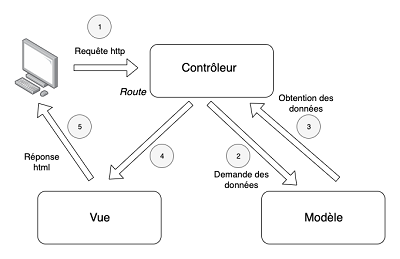
\includegraphics{Images/Modèle-vue-contrôleur_(MVC)_-_fr}
	\centering
	\caption{Rôle des trois couches logicielles du motif MVC}
\end{figure}

\subsubsection{REST}
REST (Representational State Transfer) est une architecture de messagerie utilisée par de nombreuses \gls{API} de service Web. REST est une architecture flexible, avec des instructions et la prise en charge de plusieurs normes, telles que \gls{HTTPS}, XML et . Ce dernier signifie JavaScript Object Notation, un format de données léger et minimal. \gls{JSON} est celui utilisé dans la solution pour stocker et transporter des données.

\subsubsection{DAO}
\label{DAO}
Grâce aux objets métier, le motif \gls{DAO} permet de fournir une abstraction des détails 5 du mode
de stockage. Ainsi, l’objectif du DAO peut être résumé en deux points :
\begin{enumerate}
	\item Sauvegarder les information provenant de la base de données dans des classes au lieu de laisser
	dispersés les attributs faisant partie à la même entité ;
	\item Déléguer les accès aux données persistantes à une couche à part au lieu de gérer tout dans
	le modèle. De ce fait, le reste du modèle ne serait modifié que si les règles de gestion métier
	changent.
\end{enumerate}
\textbf{Entity Framework} est utilisé faire ce motif. C'est un outil permettant de créer une couche d'accès aux données (DAL pour Data Access Layer) liées à une base de données relationnelle. Il propose la création d'un schéma conceptuel composé d'entités qui permettent la manipulation d'une source de données, sans écrire une seule ligne de SQL, grâce à LinQ To Entities. Comparé à d'autres solutions de mapping objet-relationnel (\textbf{ORM}), Entity Framework assure l'indépendance du schéma conceptuel (entités ou objets) du schéma logique de la base de données, c'est-à-dire des tables. Ainsi, le code produit et le modèle conceptuel ne sont pas couplés à une base de données spécifique. Pour en savoir plus veillez visiter le lien \href{https://pmusso.developpez.com/tutoriels/dotnet/entity-framework/introduction/}{https://pmusso.developpez.com/tutoriels/dotnet/entity-framework/introduction/}

\section{Sécurité}
Dans cette section, je présente les algorithmes et techniques de chiffrement que nous avons
utilisés pour sécuriser davantage l'application.

\subsection{Hachage des mots de passe}
Il s’avère unanime que les mots de passe représentent l’élément clé permettant aux systèmes d’information
d’authentifier les utilisateurs. De ce fait, la protection des mots de passe constitue une tâche
primordiale dans les stratégies de sécurité de toute application informatique. \newline
L’une des règles de base de la protection des mots de passe est qu’ils ne doivent pas être sauvegardés
en clair dans la base de données. Le moyen le plus fréquent pour protéger les mots de passe consiste
à sauvegarder plutôt les hash des mots de passe dans la base de données. Puis, si l’l’utilisateur saisit
son mot de passe, l’application calcule le hash et vérifie s’il existe ou non dans la base de données. Si
oui, c’est-à-dire qu’il s’agit du bon mot de passe. Sinon, cela veut dire que le mot de passe fourni est
erroné. \newline
Le calcul des hash des mots de passe est réalisé par une fonction de hachage qui désigne une
fonction à sens unique qui, à partir d’une donnée fournie en entrée, calcule une empreinte numérique,
appelée le hash, servant à identifier de façon unique la donnée en entrée. Bien évidement, les fonctions
de hachage sont nombreuses, citons à titre d’exemple :
\begin{enumerate}
	\item MD4 (R. L. Rivest, 1990) ;
	\item MD5 (R. Rivest et Dusse, 1992) ;
	\item Tiger (Anderson et Biham, 1996) ;
	\item RIPEMD (Dobbertin, Bosselaers et Preneel, 1996) ;
	\item Whirlpool (Barreto et Rijmen, 2000) ;
	\item MD6 (R. L. Rivest et al., 2008) ;
	\item BLAKE (Aumasson et al., 2008) ;
	\item la famille SHA (Michail et al., 2005 ; Glabb et al., 2007 ; Dworkin, 2015) ;
	\item GOST (Dolmatov et Degtyarev, 2013).
	\newline
\end{enumerate}
Certaines de ces fonctions de hachage sont actuellement vulnérables car elles ont été déjà cassées
et ne sont plus résistantes aux collisions \footnote{Dans notre contexte, une collision désigne deux mots de passe différent ayant le même hash.} (Chabaud et Joux, 1998 ; Wang et Yu, 2005 ; Wang, Yin et Yu, 2005 ; Mendel et al., 2008). Nous avons choisi \textbf{SHA-256} comme elle n’a, jusqu’à présent, pas été compromise par une attaque significative.

\section{Autres}
Dans cette section, je présente tout d’abord l’environnement de rédaction puis le logiciel de sauvegarde et de partage des fichiers.
\subsection{Environnement de rédaction : MikTex \& TexStudio}
Dans cette section, j'explique tout d’abord ce que signifie Tex puis LaTeX. Ensuite, je présente la distribution Tex et l’éditeur LaTeX que j'ai utilisé. Enfin, j'argumente pourquoi j'ai choisi LaTeX. \newline
En effet, TeX est un langage et un système de composition de documents. Il fournit de nombreuses commandes permettant de spécifier le format du document avec beaucoup de détails \footnote{Styles de police, espacement, crénage, ligatures, etc.}et dispose d’algorithmes spécialisés pour le calcul de flux optimal de texte dans les documents \footnote{Par exemple, où s’achèvent les lignes, les pages, etc.}. TeX met donc à disposition des algorithmes et des commandes puissants pour spécifier les moindres détails lors de l’élaboration d’un document. Mais, vu que l’utilisation directe du TeX est assez ardue, il a été étendu en LaTeX qui constitue un jeu de macro-commandes basées sur TeX. \newline
L’idée sur laquelle se base LaTeX est de cacher la complexité de la mise en page en séparant le format (mise en page) du contenu du document. Ainsi, il suffit de donner une structure au contenu du document sans besoin de rentrer dans les détails. Par exemple, pour créer une nouvelle section, il n’est demandé que d’écrire \textbf{\ section\{...\}} au lieu de sélectionner une police, définir son style, insérer les espaces
appropriés avant et après l’en-tête de section, etc. Tous ces détails seront gérés automatiquement par TeX. \newline 
Pour pouvoir travailler sur LaTeX, il faut tout d’abord choisir une distribution TeX puis un éditeur LaTeX. Bien évidement, les distributions TeX sont nombreuses ainsi que les éditeurs LaTeX. La distribution Tex que j'ai utilisé est \textbf{MikTex} et j'ai utilisé \textbf{TeXStudio} comme éditeur LaTeX. \newline
J'ai privilégié LaTeX au détriment de Microsoft Office non seulement parce que LaTeX est gratuit et multiplateforme tandis que Microsoft Office est payant et n’est natif que sur Windows mais aussi pour les raisons suivantes :
\begin{enumerate}
	\item La gestion automatique de la mise en page en LaTeX du document via les templates ;
	\item La gestion automatique des références bibliographiques (via BibTex par exemple) ;
	\item La génération automatique et en une seule commande de tables de matières, liste de figures et liste de tableaux ;
	\item La génération automatique de la liste des acronymes cliquables tout en précisant les pages où figurent chaque acronyme ;
	\item La taille des document produits par LaTeX fait généralement la moitié de leurs équivalents sur Microsoft Word ;
\end{enumerate}

\subsection{Logiciel de sauvegarde et de partage : Dropbox}
Pour pouvoir travailler sur le projet à distance, j'avais besoin d’un moyen nous permettant non seulement de sauvegarder les documents issus du projet mais aussi de pourvoir les partager avec notre encadrant et les membres du groupe. Pour ce faire, j'avais le choix entre utiliser un service de messagerie électronique \footnote{Il s’agit de partager les documents par e-mail.} ou faire recours à un service d’hébergement de fichiers. J'ai opté pour ce dernier car il m'a permis de pouvoir travailler sur le même espace de travail avec une synchronisation de modifications en temps réel. \newline
Bien évidement, les services d’hébergement de fichiers sont nombreux : Google Drive, Microsoft OneDrive, Dropbox, pCloud, etc. J'ai choisi Dropbox comme je m'y suis déjà habitué.